\section{Исследование природы фона и выделение сигнала}

Для исследования природы фона были использованы события, сгенерированные методом Монте-Карло. Для соответствия отобранным данным критерии отбора были выбраны аналогичными. Также была выполнена дополнительная операция — фитирование по массе и по вершине.

Среди множества идентифицированных дочерних продуктов распада частицы $\xi$ можно использовать известные свойства импульсов этих продуктов, исходящих из вершины распада, для корректировки измеренных импульсов. Это позволяет улучшить точность, соответствуя гипотезе (далее этот метод будет называться «фитом в вершину»). Аналогично, исходя из известной инвариантной массы для $\xi$, импульсы дочерних частиц могут быть скорректированы так, чтобы $M_p = \sqrt{\sum_n \inner{p_n}_\gamma \inner{p_n}^\gamma}$ совпадала с $M^{\text{real}}_{\xi}$, где $p_n$ — 4-импульс, соответствующий $d_n$. Этот метод будет называться «фитом в массу». Для этих целей использовались алгоритмы фита в вершину и массу, принятые в коллаборации KEK.

В результате отбора было получено распределение восстановленной массы $\Lambda_c$ (рис. \ref{MC_inc_ful}).

\begin{figure}[H]
    \centering
    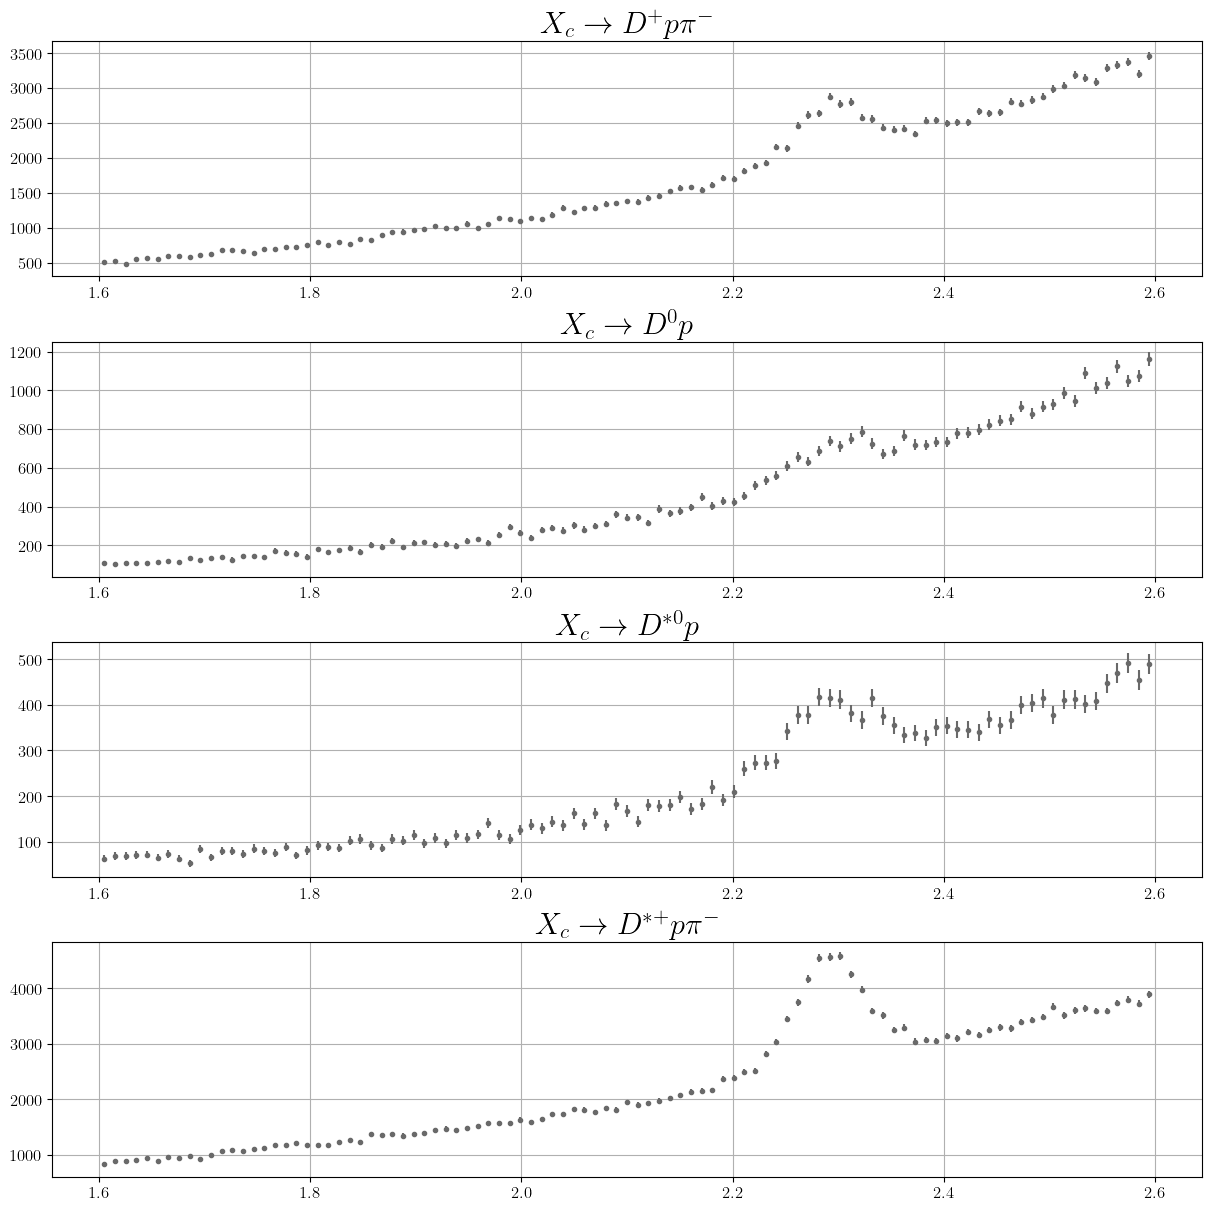
\includegraphics[width=1\linewidth]{img/MC_inc.png}
    \caption{Распределение количества событий по каналам.}
    \label{MC_inc_ful}
\end{figure}

Также в этих событиях была выделена энергия $\Lambda_c$ (если она присутствует); если нет, то $E_{\Lambda_c} = 0$ соответственно.

Для выделения сигнальных событий проводится проверка:

\begin{itemize}
    \item Каждая детектируемая частица правильно идентифицирована, то есть треку была присвоена верная гипотеза на основе информации из Монте-Карло.
    \item $\abs{E_{\text{beam}} - E_{X_c} - E_{\Lambda_c}} < 0.015$ ГэВ, где $E_{\text{beam}}$ — энергия пучков.
    \item Проверяется, что каждая комбинированная частица действительно существовала и распалась по предполагаемому каналу, а дочерние частицы правильно присвоены.
\end{itemize}

В итоге получаем распределение (рис. \ref{MC_sig}).

\begin{figure}[H]
    \centering
    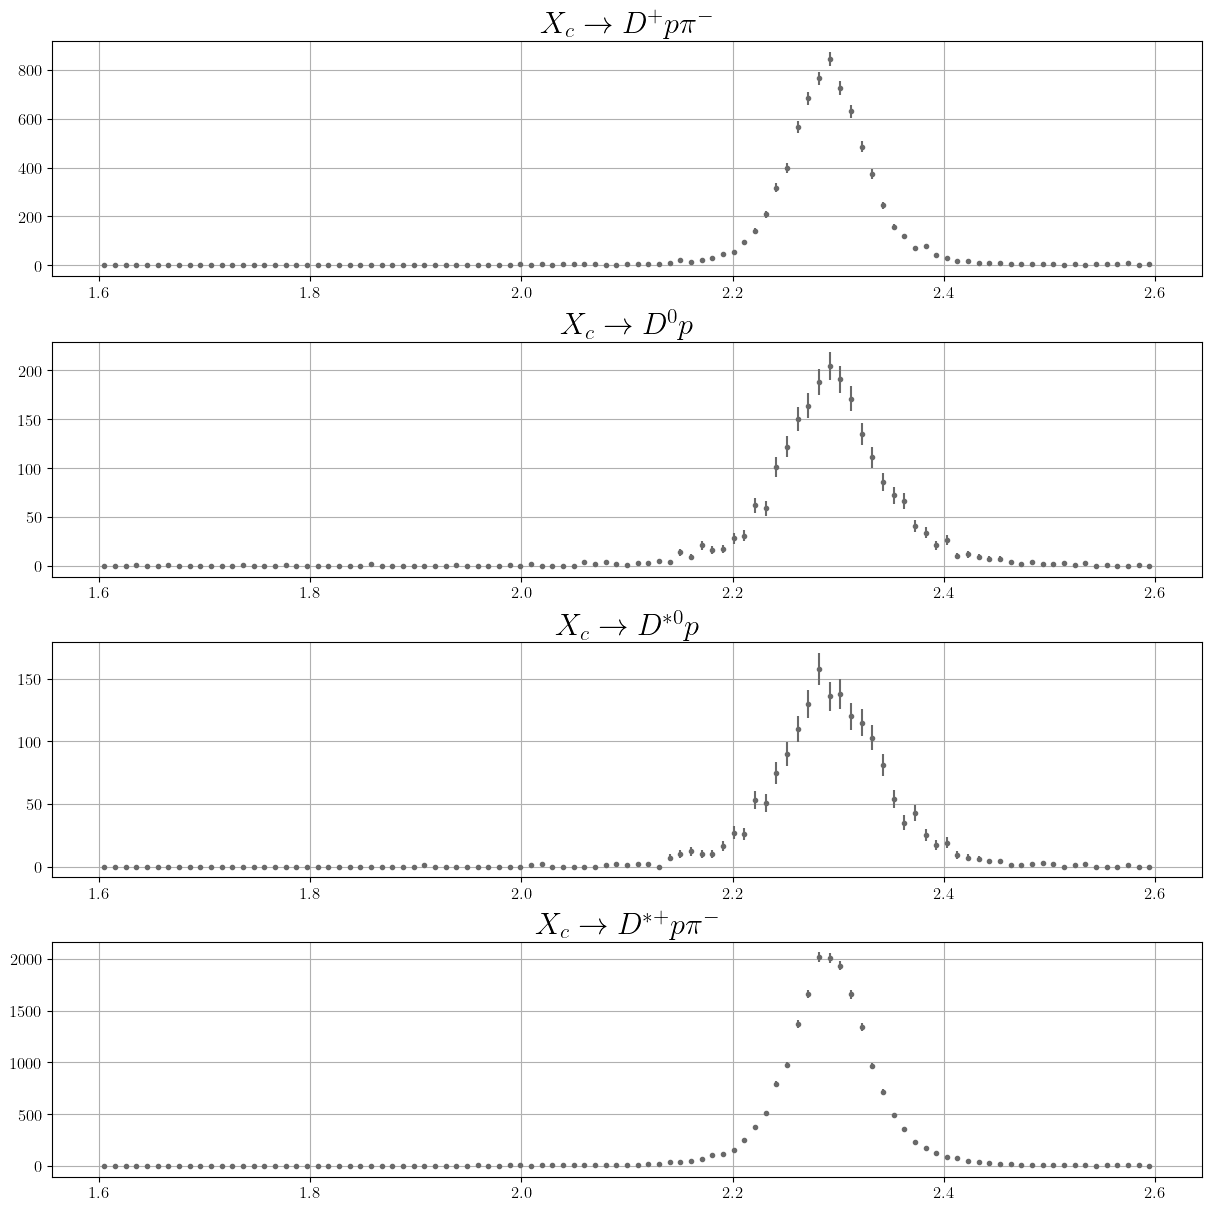
\includegraphics[width=1\linewidth]{img/MC_sig.png}
    \caption{Распределение сигнальных событий по каналам.}
    \label{MC_sig}
\end{figure}

Распределение аппроксимировалось функцией из трёх гауссианов для каналов с заряженными треками и из двух гауссианов для каналов с нейтральными треками с произвольной нормировкой (где $N$ — количество событий, вычисленное методом максимального правдоподобия, $N_r$ — истинное количество событий). Использование нескольких гауссианов обусловлено различием разрешения каналов $D$-мезонов:

\begin{equation}
    f_{\text{sig}} = C_{\text{sig}}\sum_{i=1}^{2,3} A_i N_i(x)
\end{equation}

где $\sum_i A_i = 1$ для сохранения нормировки. Итог аппроксимации (рис. \ref{MC_sig_fit}).

\begin{figure}[H]
    \centering
    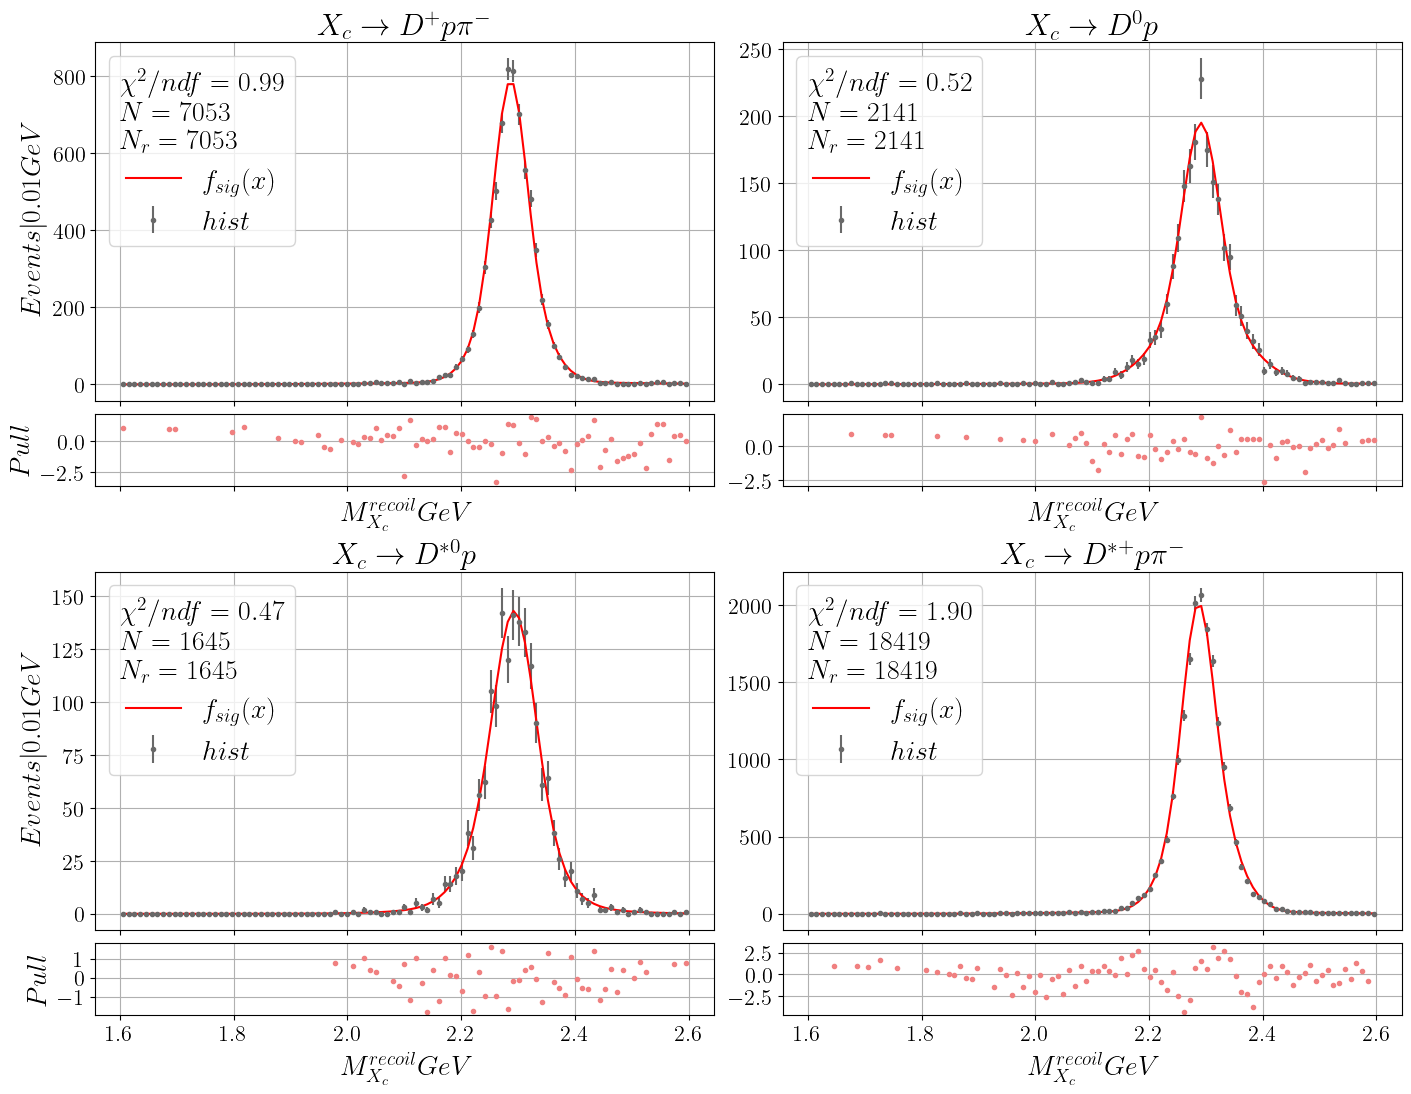
\includegraphics[width=1\linewidth]{img/MC_sig_fit.png}
    \caption{Распределение сигнальных событий по каналам.}
    \label{MC_sig_fit}
\end{figure}

Помимо сигнала рассматриваются два вида фоновых событий. Первый описывает потери в детекторе с критериями отбора:

\begin{itemize}
    \item Каждая детектируемая частица правильно идентифицирована, то есть треку была присвоена верная гипотеза на основе информации из Монте-Карло.
    \item $E_{\text{beam}} - E_{X_c} - E_{\Lambda_c} > 0.015$ ГэВ.
\end{itemize}

В итоге получено распределение (рис. \ref{MC_bg_lost}).

\begin{figure}[H]
    \centering
    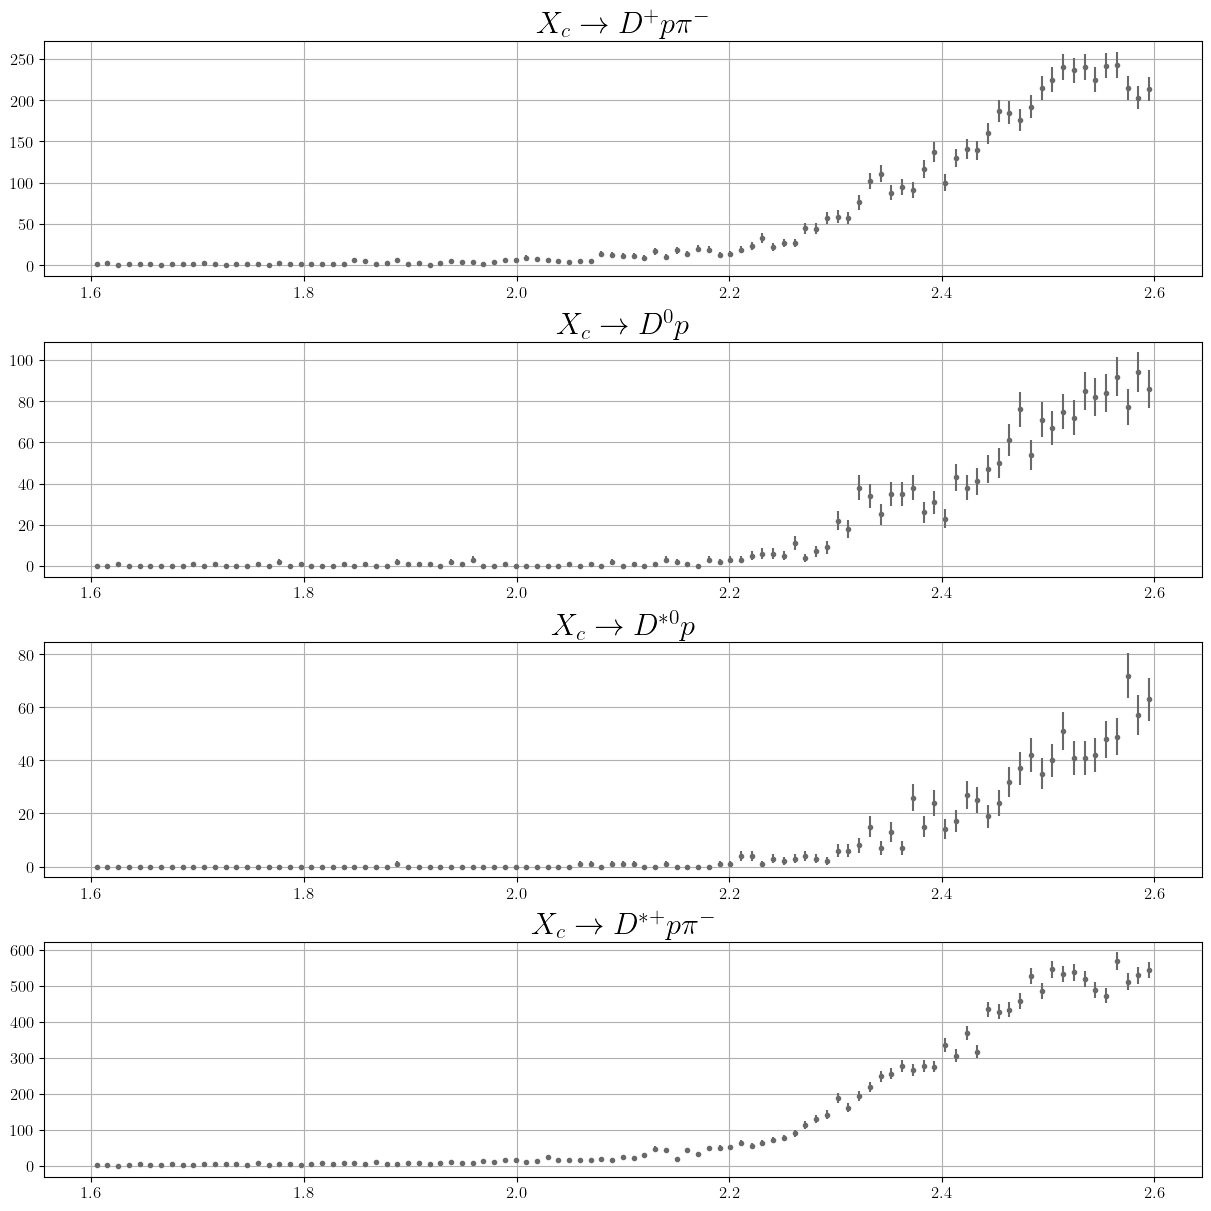
\includegraphics[width=1\linewidth]{img/MC_sqr_bg.png}
    \caption{Распределение событий с потерями.}
    \label{MC_bg_lost}
\end{figure}

Распределение показывает рост от $M_{\Lambda_c}$, так как если частица потеряна, то восстановленная масса должна быть:

\begin{equation}
    p_{X_c} + p_{\Lambda_c} + p_{\text{lost}} = p_{\text{beam}} \implies \abs{p_{\text{beam}} - p_{X_c}} = \abs{p_{\Lambda_c} + p_{\text{lost}}}
\end{equation}

Для описания распределения использовались два корня, начинающих рост от $M_{\Lambda_c}$ (потеря фотона) и $M_{\Lambda_c} + M_{\pi^0}$ (потеря $\pi^0$-мезона). Размытие распределений согласовано с размытием пика сигнала, и корни свёртываются с функцией распределения сигнала. В итоге распределение аппроксимировалось функцией:

\begin{equation}
    F_{\text{lost}} = C_{\text{lost}} \int f_{\text{sig}}(x)\cdot f_{\text{lost}}(x-s) dx
\end{equation}

где

\begin{equation}
    f_{\text{lost}}(x) = c_1\sqrt{\inner{x - M_{\pi}} \cdot \theta\inner{x - M_{\pi}}} + c_2\sqrt{x \cdot \theta\inner{x}}
\end{equation}

Результат подгонки (рис. \ref{MC_bg_lost_fit}).

\begin{figure}[H]
    \centering
    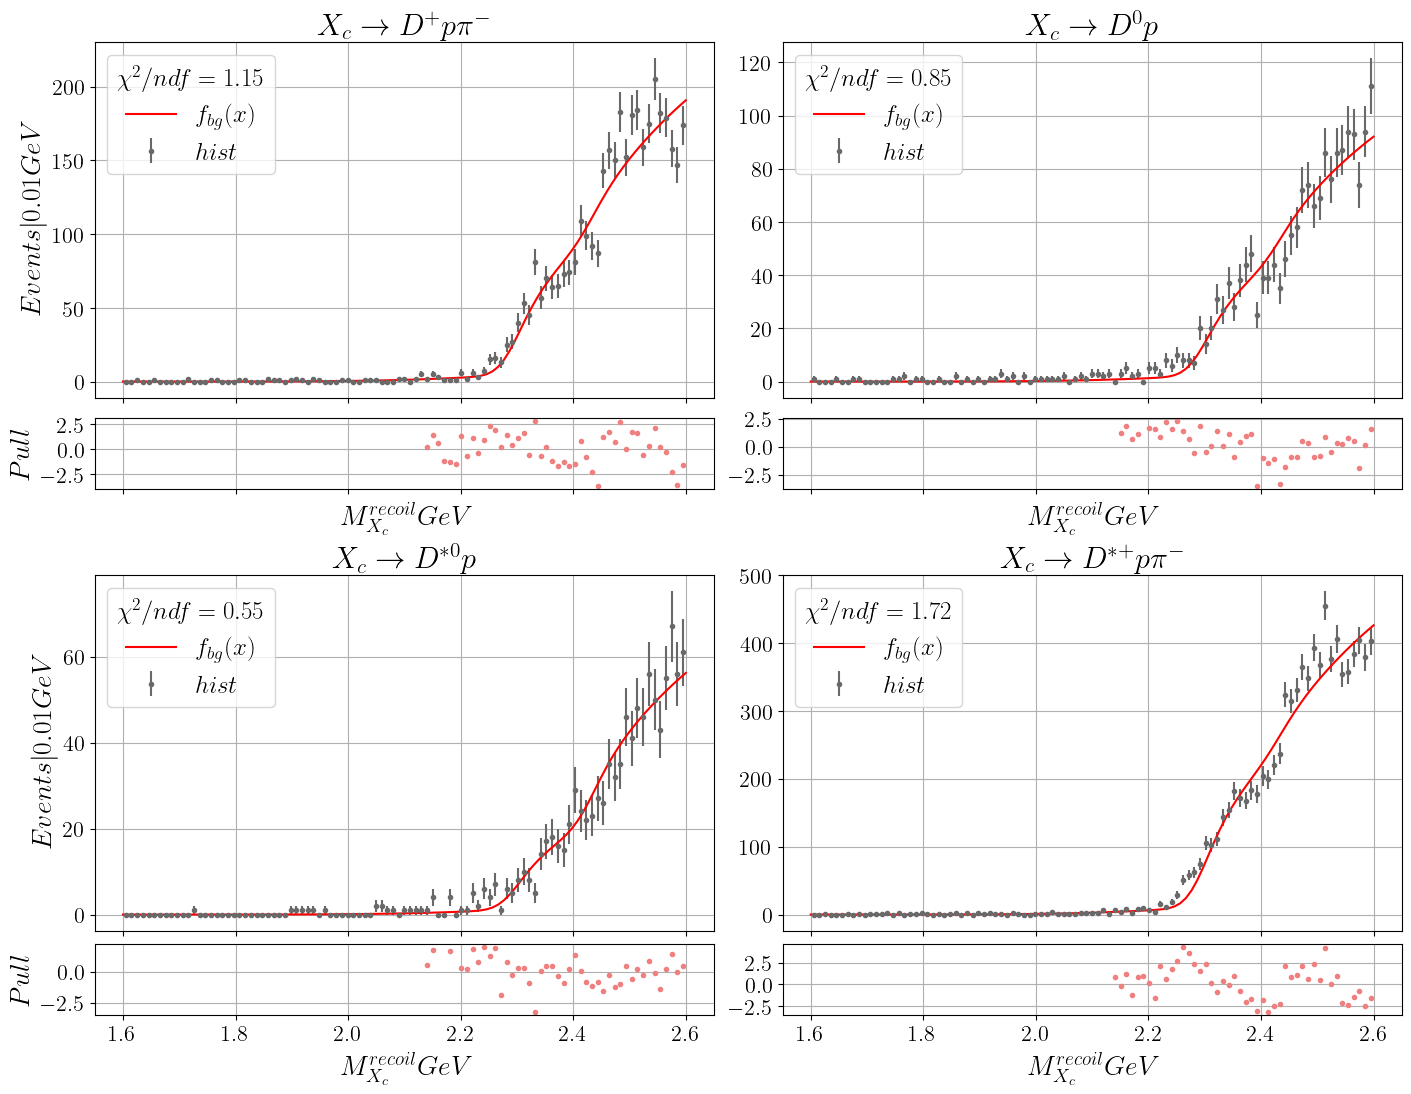
\includegraphics[width=1\linewidth]{img/MC_sqr_bg_fit.png}
    \caption{Распределение событий с потерями.}
    \label{MC_bg_lost_fit}
\end{figure}

Второй вид фона — комбинаторный, его распределение представлено на рис. \ref{MC_comb}.

\begin{figure}[H]
    \centering
    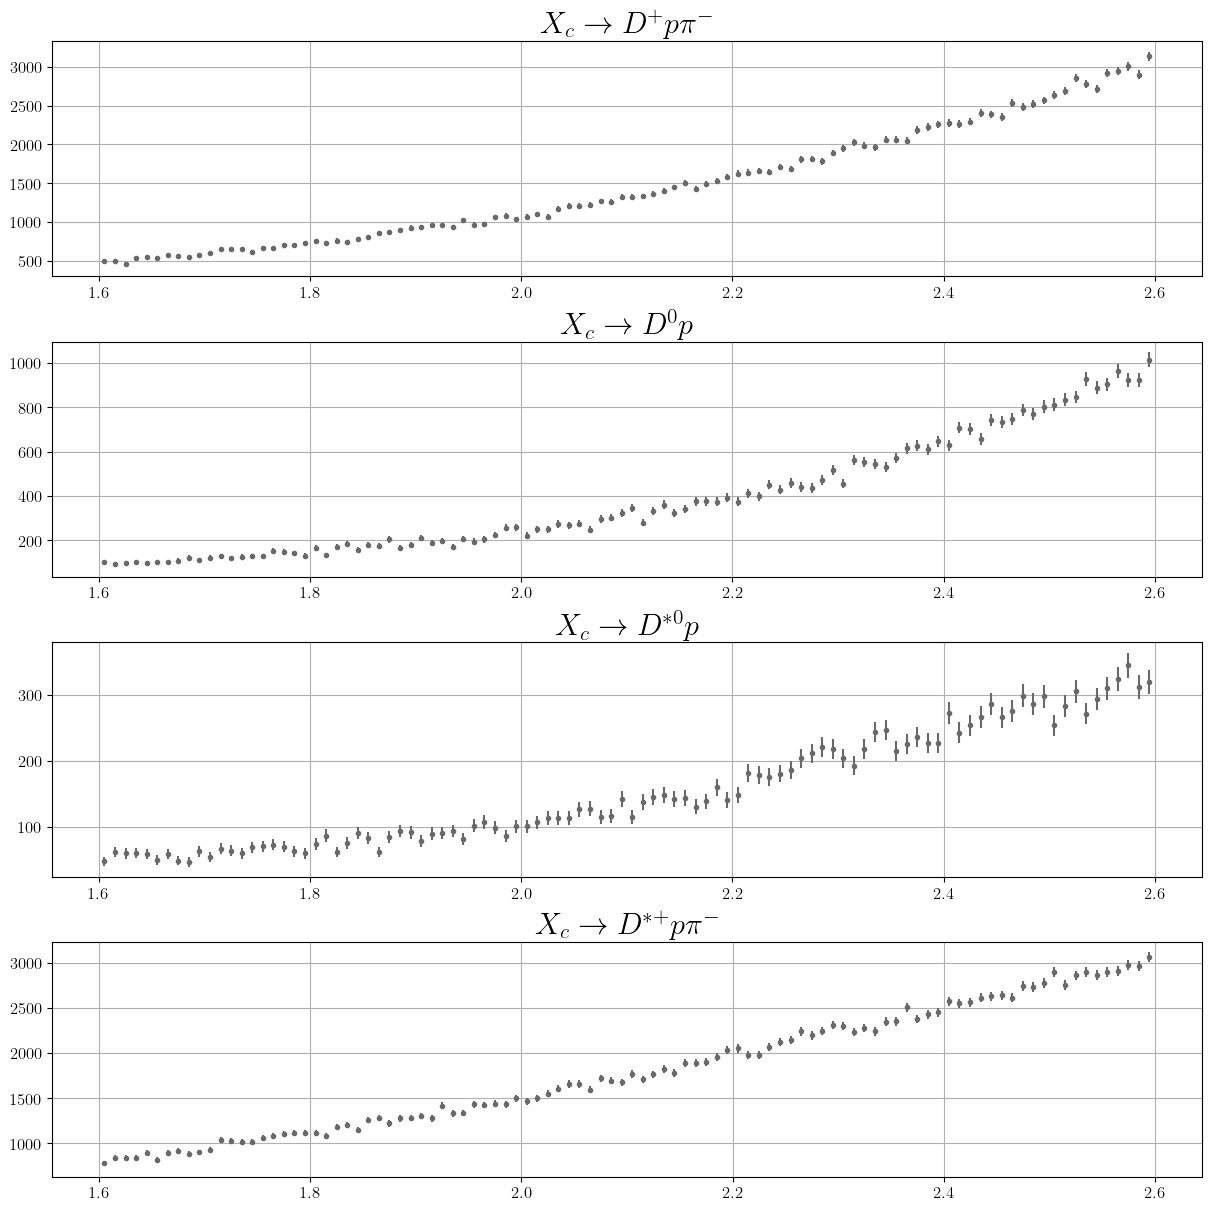
\includegraphics[width=1\linewidth]{img/MC_comb.png}
    \caption{Распределение событий комбинаторного фона.}
    \label{MC_comb}
\end{figure}

Комбинаторный фон стандартно описывается экспонентой, так как вероятность ошибочной идентификации частиц и формирования $X_c$ увеличивается с количеством частиц в событии. Для улучшения описания в распределение добавлен линейный полином.

Аппроксимация распределения выполнялась функцией:

\begin{equation}
    F_{\text{comb}} = \exp\insqr{\inner{x - \mu}\lambda} + c_0 + c_1 x
\end{equation}

Результат подгонки (рис. \ref{MC_comb_fit}).

\begin{figure}[H]
    \centering
    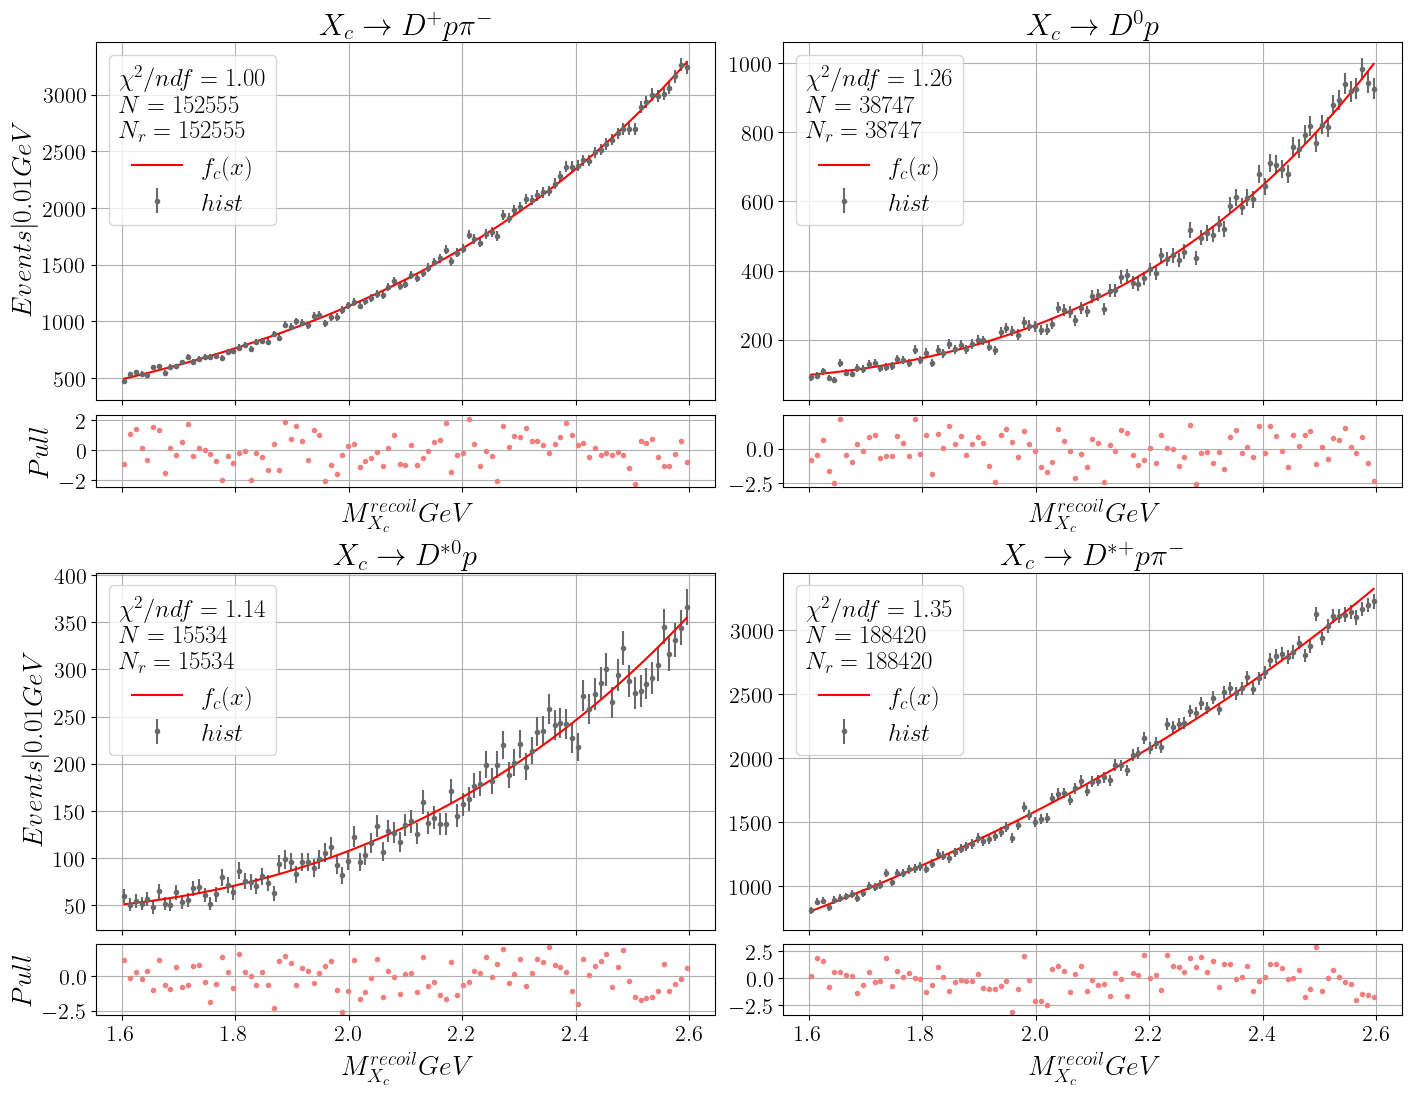
\includegraphics[width=1\linewidth]{img/MC_comb_fit.png}
    \caption{Распределение событий комбинаторного фона.}
    \label{MC_comb_fit}
\end{figure}
